\section{Introduction}

The honeycomb maze is a development from the 'T maze', 'star maze' and Morris water maze

INSERT FIGURES FOR THESE TYPES OF MAZES
\begin{figure}
    \centering
    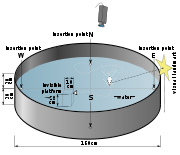
\includegraphics[scale = 0.7]{images/morris_water_maze.png}
    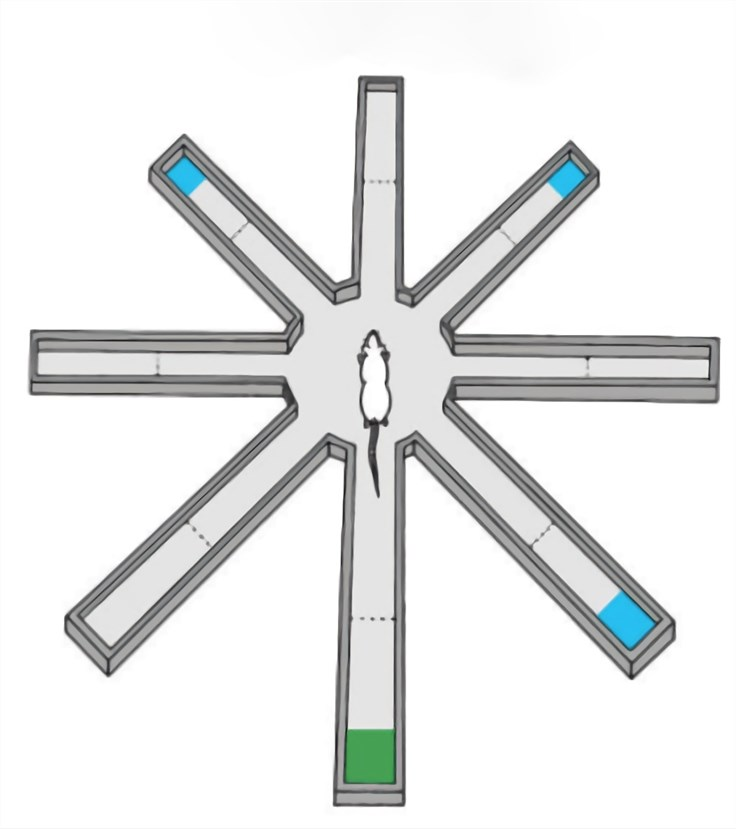
\includegraphics[scale = 0.25]{images/radial_arm_maze.jpg}
    \caption{Selection of Mazes that have previously been used to investigate how mice encode space in the brain}
    \label{fig:previousmazes}
\end{figure}

The honeycomb maze is an development on the $6 \times 6$ honeycomb maze which is very important in the investigation of hippocampal place cells and their role in how mouse brains are able to encode information about where they are located in space. 

However, there are many limitations to using the static honeycomb maze: The cost associated with building and using this maze are very high. This means that the experimentation tool is very inaccessible to smaller  laboratories. The number of platforms (ie, the area over which the mouse can traverse), is limited. This means  
